\section{Planen}


\begin{frame}[c]{Planen}
    \normalsize
    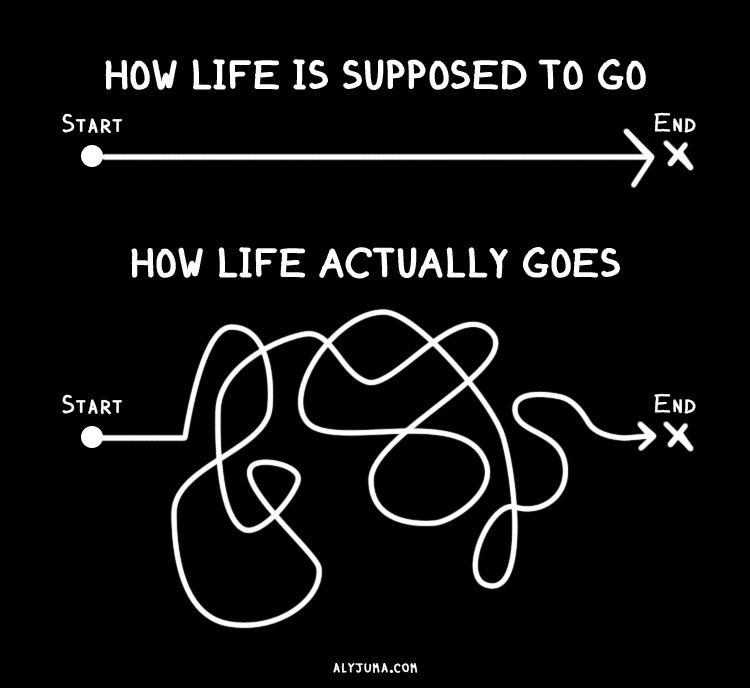
\includegraphics[height=0.9\textheight]{lifepath}
    Bild von \cite{lifepath-pic}
\end{frame}


\begin{frame}[c]{Warum Planen}
    Man möchte Verstehen:
    \begin{itemize}[<+(1)->]
        % \item Versuch, das Ziel zu verstehen
        \item \textbf{Wann} das Ziel erfüllt ist
        \item \textbf{Wie} das Ziel erreicht werden kann
        \item Welche \textbf{Hindernisse} auf dem Weg sind
        \item Was die \textbf{nächsten Schritte} sind
        \item Die \textbf{Gesamtsituation}
    \end{itemize}
\end{frame}

\subsection{Ziele Definieren}


\subsection{Leit- und Verzögerungsmaße}
% Leitmaß & Verzögerungsmaß


\subsection{Nächste Schritte}


